% Created 2023-04-09 Sun 21:10
% Intended LaTeX compiler: pdflatex
\documentclass[presentation,aspectratio=169]{beamer}
\usepackage[utf8]{inputenc}
\usepackage[T1]{fontenc}
\usepackage{graphicx}
\usepackage{grffile}
\usepackage{longtable}
\usepackage{wrapfig}
\usepackage{rotating}
\usepackage[normalem]{ulem}
\usepackage{amsmath}
\usepackage{textcomp}
\usepackage{amssymb}
\usepackage{capt-of}
\usepackage{hyperref}
\usepackage{khpreamble, euscript}
\DeclareMathOperator{\atantwo}{atan2}
\newcommand*{\ctrb}{\EuScript{C}}
\newcommand*{\obsv}{\EuScript{O}}
\usetheme{default}
\author{Kjartan Halvorsen}
\date{\today}
\title{Odometría}
\hypersetup{
 pdfauthor={Kjartan Halvorsen},
 pdftitle={Odometría},
 pdfkeywords={},
 pdfsubject={},
 pdfcreator={Emacs 26.3 (Org mode 9.4.6)}, 
 pdflang={English}}
\begin{document}

\maketitle

\section{Differential drive}
\label{sec:org2694e9d}

\begin{frame}[label={sec:org35aaf78}]{Robot móvil - modelo canónico}
\begin{columns}
\begin{column}{0.4\columnwidth}
\begin{center}
 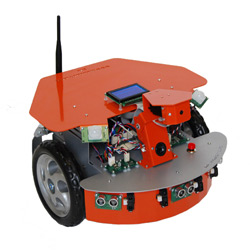
\includegraphics[width=.3\linewidth]{../figures/X80Pro.jpg}
\end{center}
\begin{center}
 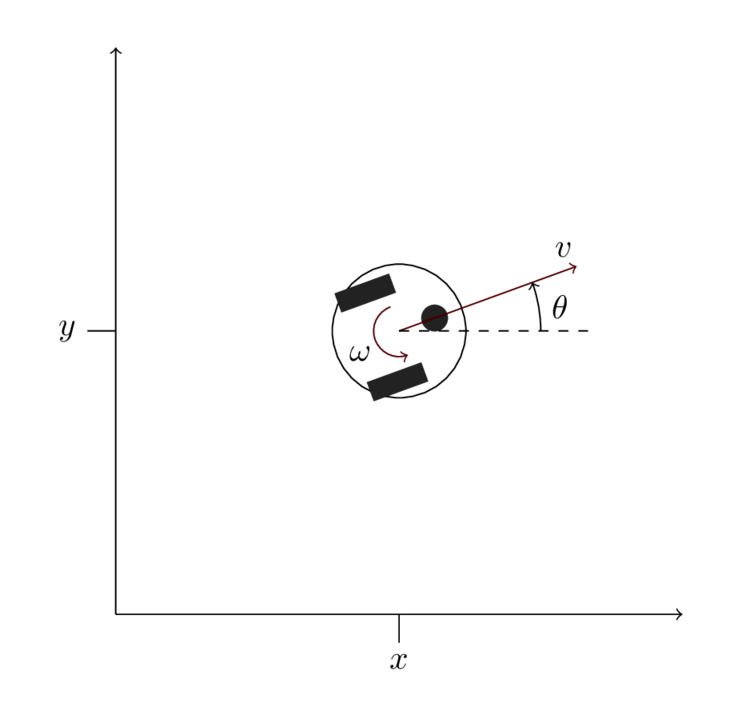
\includegraphics[width=1.0\linewidth]{../figures/unicycle-model}
\end{center}
\end{column}

\begin{column}{0.6\columnwidth}
\pause


\[ \xi = \begin{bmatrix} \theta\\x\\y \end{bmatrix},   \quad u = \begin{bmatrix} \omega\\v \end{bmatrix}\]



\[\frac{d}{dt} \xi = \begin{bmatrix} \dot{\theta}\\\dot{x}\\\dot{y} \end{bmatrix} = \begin{bmatrix} \omega\\ v\cos\theta\\v\sin\theta\end{bmatrix} \]
\end{column}
\end{columns}
\end{frame}

\begin{frame}[label={sec:org076c512}]{El método de Euler para integración numérica}
Dado ecuación diferencial (posiblemente no-lineal y variante en el tiempo)
\[ \frac{d}{dt} y = f(y,t, u) \]
y valor inicial \(y(t_k) = y_k\),
el valor de la función \(y(t_{k+1}) = y(t_k + \Delta t)\) se puede estimar con

\[\hat{y}(t_{k+1}) = y_k + \Delta t \;f\big(y_k, t_k, u(t_k)\big). \]
\end{frame}





\begin{frame}[label={sec:orgecf02f4}]{Integrando el modelo cinemático}
\small

\begin{columns}
\begin{column}{0.4\columnwidth}
\begin{center}
 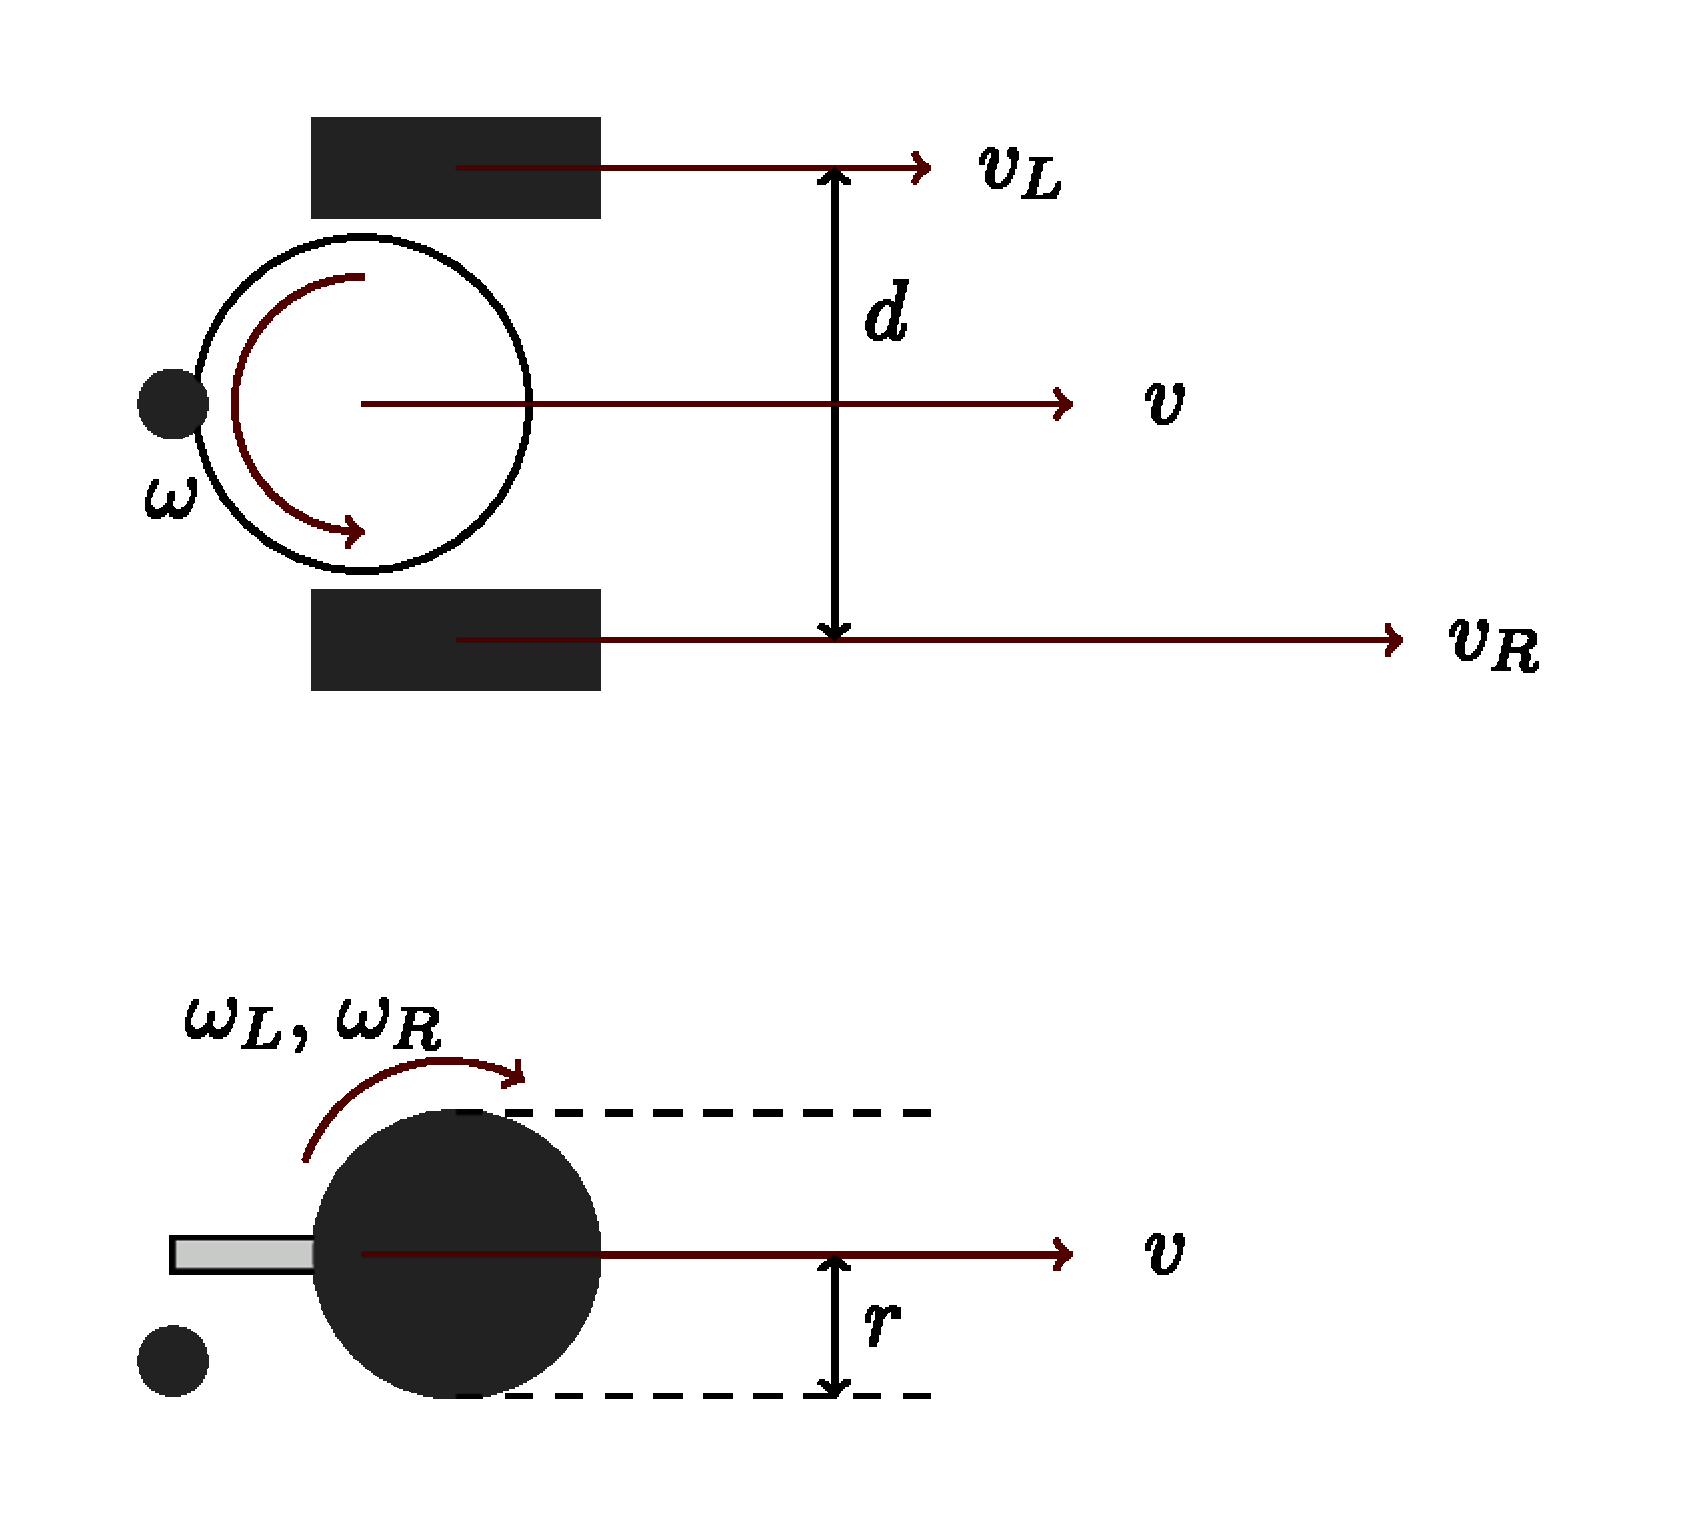
\includegraphics[width=1.0\linewidth]{../figures/unicycle-model-details}
\end{center}
\end{column}

\begin{column}{0.6\columnwidth}
\[ \xi = \begin{bmatrix} \theta\\x\\y \end{bmatrix},   \quad u = \begin{bmatrix} \omega\\v \end{bmatrix}\]
\[\frac{d}{dt} \xi = \begin{bmatrix} \dot{\theta}\\\dot{x}\\\dot{y} \end{bmatrix} = \begin{bmatrix} \omega\\ v\cos\theta\\v\sin\theta\end{bmatrix} \]

\pause

\alert{Actividad} Aplica el método de Euler!

\[\hat{y}(t_{k+1}) = y_k + \Delta t \; f\big(y_k, t_k, u(t_k)\big). \]
\end{column}
\end{columns}
\end{frame}


\begin{frame}[label={sec:orgd12ceab}]{Una mejor approximación}
\begin{columns}
\begin{column}{0.6\columnwidth}
\begin{center}
  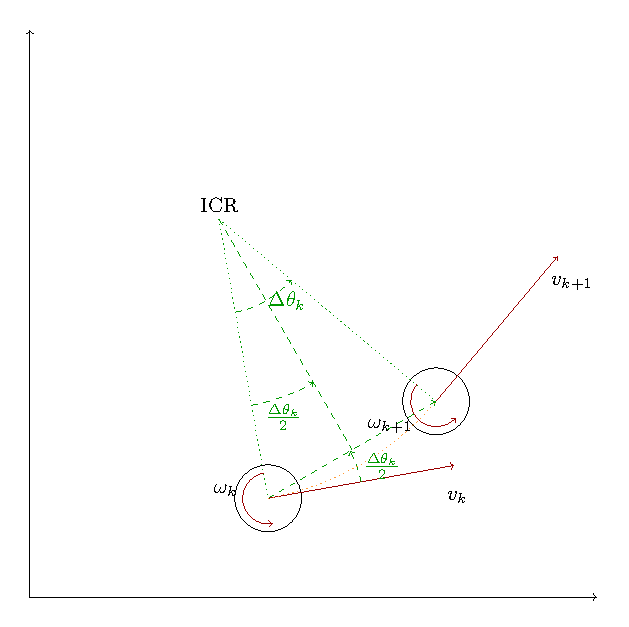
\includegraphics[width=\linewidth]{../figures/odometry-improvement}
\end{center}
\end{column}

\begin{column}{0.4\columnwidth}
\begin{itemize}
\item Con velocidad angular y linear constante, la trayectoria es un arco de un circulo, con un sector \[\Delta \theta = \omega_k \Delta t.\]
\item La dirección \(\theta_k + \frac{\Delta \theta}{2}\) da la vector hacía la nueva posición.
\[\vec{v}_{k, corr} = \begin{bmatrix} v_k \cos(\theta_k + \frac{\Delta \theta}{2})\\v_k\sin(\theta_k + \frac{\Delta \theta}{2})\end{bmatrix}\]
\end{itemize}
\end{column}
\end{columns}
\end{frame}
\end{document}